\documentclass[a4paper]{article} % For LaTeX2e
\usepackage{nips15submit_e,times}
\usepackage{hyperref}
\usepackage{url}
\usepackage{amsmath,amssymb,graphicx,booktabs}

% Course-required: use NIPS camera-ready format.
% The bundled NIPS 2015 style defaults to US Letter, while the assignment
% requires A4 pages.
\setlength{\paperwidth}{210mm}
\setlength{\paperheight}{297mm}
\pdfpagewidth=\paperwidth
\pdfpageheight=\paperheight
\nipsfinalcopy

\title{Quantile-Initialised Ordinal Collaborative Filtering\\ with Gated Auxiliary Fusion}
\author{
  Kevin Zhu \\ Australian National University \\ \texttt{u7338066@anu.edu.au}
}

\begin{document}
\maketitle

\begin{abstract}
We propose a simple calibration recipe for cumulative-link collaborative
filtering: initialise the monotone thresholds from the empirical rating
quantiles of the training set, parameterise their spacing through a
softplus-inverse, and exclude them from $L_2$ regularisation. The recipe
matches the data marginal at training start and gives a native rating
distribution without sacrificing RMSE. Paired with per-dimension gated fusion
of side information, the gated$+$ordinal configuration attains
RMSE $0.9124\pm0.0036$ and NLL $1.2584$ across the five canonical
MovieLens-100K splits, beating both a no-fusion MF analogue ($0.9160$) and
additive fusion ($0.9189$) on the across-split RMSE mean. A MovieLens-1M
scale-up preserves the same ordering (RMSE $0.8481\pm0.0006$,
NLL $1.184$). The contribution is practical rather than algorithmic:
standard components are combined into a reproducible, calibrated recommender
pipeline.
\end{abstract}

\section{Introduction}
\label{sec:intro}

Collaborative filtering (CF) for explicit feedback predicts unobserved user--item
ratings from a sparse matrix. Latent-factor models based on matrix
factorisation~\cite{koren2009mf} remain standard baselines and building blocks
on MovieLens~\cite{harper2015movielens}.
Two persistent issues remain when these models are applied as a course-style
data-analytics tool rather than a production recommender. First, side
information (user demographics, item genres) is typically injected by adding a
projected feature vector to the latent embedding, with no learned mechanism to
decide \emph{when} to trust the embedding versus the side information. Second,
the rating is treated as a continuous quantity even though it is in fact a
five-class ordinal variable; the resulting predictions can be RMSE-competitive
yet badly calibrated as distributions over star ratings.

\paragraph{Related work and contribution.}
The two issues above have been addressed separately: gated content fusion is
used by GATE~\cite{ma2019gate}, while cumulative-link ordinal regression starts
from McCullagh's model~\cite{mccullagh1980ordinal} and appears in recommenders
such as OrdRec~\cite{koren2011ordrec}, OrdNMF~\cite{gouvert2020ordnmf}, and
OPRFM~\cite{zaman2025oprfm}. Our contribution is implementation-level rather
than algorithmic: we combine gated side-information fusion with a calibrated
cumulative-link head on a transparent MF core, and we separate their effects
through ablations, calibration plots, cold-start analysis, and a small
MovieLens-1M scale-up.

\section{Problem Definition}
\label{sec:problem}

Let $\mathcal{U}=\{1,\dots,n\}$ be the set of users and $\mathcal{I}=\{1,\dots,m\}$
the set of items. Observed ratings form a sparse set
$\mathcal{D}=\{(u_t,i_t,r_t)\}_{t=1}^{N}$ with $r_t\in\{1,2,3,4,5\}$. Each user
$u$ carries a side-information vector $f_u\in\mathbb{R}^{d_u}$ (z-scored age,
one-hot gender, one-hot occupation in MovieLens-100K, $d_u=24$) and each
item $i$ carries $g_i\in\mathbb{R}^{d_i}$ (multi-hot genre indicator,
$d_i=19$). The task
is to predict $\hat r_{ui}$ for held-out $(u,i)$ pairs, evaluated by RMSE, MAE,
classification accuracy of the rounded prediction, and where applicable the
held-out negative log-likelihood (NLL) of the predicted rating distribution.

\section{Method}
\label{sec:method}

\subsection{Matrix factorisation backbone}
We start from a biased dot-product MF model. Each user and item carries a
$d$-dimensional embedding ($p_u, q_i\in\mathbb{R}^d$) and a scalar bias
($b_u, b_i\in\mathbb{R}$). The pre-head score is
\begin{equation}
\label{eq:score}
s_{ui} \;=\; p'_u \cdot q'_i \;+\; b_u \;+\; b_i,
\end{equation}
where $p'_u,q'_i$ are the (possibly fused) representations defined below. With
fusion disabled, $p'_u\equiv p_u$ and $q'_i\equiv q_i$.

\subsection{Gated auxiliary fusion}
\label{sec:method:fusion}
Let $a_u=\mathrm{ReLU}(W_u f_u + b_{f,u})$ be a learned projection of the user
side features into the embedding space, and similarly $a_i=\mathrm{ReLU}(W_i g_i + b_{f,i})$
for items. We define the fused user representation as
\begin{equation}
\label{eq:gate}
g_u \;=\; \sigma\!\left(W_g \,[\,p_u \,\Vert\, a_u\,] + b_g\right),\qquad
p'_u \;=\; (\mathbf{1}-g_u)\odot p_u \;+\; g_u\odot a_u,
\end{equation}
where $\Vert$ denotes concatenation and $\odot$ is the Hadamard product, so the
gate $g_u\in[0,1]^d$ acts \emph{per dimension}. The item-side fusion is
identical with $(q_i,a_i)$ in place of $(p_u,a_u)$. We zero-initialise both
$W_g$ and $b_g$, which makes $g_u\equiv \tfrac12\mathbf{1}$ at training start.
This gives every dimension the same neutral starting mixture between the ID
embedding and the ReLU-projected side features; the gate then opens and closes
per dimension as gradient flows. As an ablation we also consider the
\emph{additive} variant $p'_u = p_u + a_u$ and the \emph{none} variant
$p'_u\equiv p_u$ (and similarly for items).

\subsection{Ordinal regression head}
\label{sec:method:head}
For the head we treat $r$ as an ordinal variable with $K=5$ classes. We use the
cumulative-link model of McCullagh~\cite{mccullagh1980ordinal} with monotone
thresholds $\theta_1<\theta_2<\theta_3<\theta_4$:
\begin{equation}
\label{eq:cum}
P(r\le k\mid s) = \sigma(\theta_k - s),\qquad
P(r=k\mid s) = \sigma(\theta_k - s)-\sigma(\theta_{k-1} - s),
\end{equation}
with $\theta_0=-\infty$ and $\theta_5=+\infty$. We enforce monotonicity by the
softplus reparameterisation
\begin{equation}
\label{eq:softplus}
\theta_k=\theta_1+\sum_{j=1}^{k-1}\mathrm{softplus}(\delta_j),
\end{equation}
which guarantees $\theta_k<\theta_{k+1}$ for any unconstrained parameters.

\paragraph{Empirical-quantile initialisation (the recipe).}
We initialise from the empirical
rating distribution. Let $\hat p_k$ be the training-set frequency of rating
$k$ and $\hat F_k=\sum_{j\le k}\hat p_j$ its cumulative. Choosing
\begin{equation}
\label{eq:quantile-init}
\theta_k = \mathrm{logit}(\hat F_k),\qquad
\delta_j = \log\!\bigl(\exp(\theta_{j+1}-\theta_j) - 1\bigr)
\end{equation}
guarantees $P(r{\le}k\mid s{=}0)=\hat F_k$, so the predicted marginal at the
start of training equals the data marginal exactly. The second equation is
just the softplus inverse, recovering the unconstrained $\delta_j$ that the
optimiser then updates. We also exclude $\{\theta_1,\delta_j\}$ from weight
decay because their scale carries calibration information.

The training loss is the negative log-likelihood
$\mathcal{L}_{\mathrm{ord}}=-\frac{1}{N}\sum_t \log P(r=r_t\mid s_{u_ti_t})$,
and the point prediction is the expected rating
$\hat r_{ui}=\sum_{k=1}^{5}k\,P(r=k\mid s_{ui})$. As an ablation we also
consider the standard \emph{sigmoid} head:
$\hat r_{ui}=4\sigma(s_{ui})+1$ trained with mean-squared error.

\subsection{Complexity}
\label{sec:complexity}
The MF backbone has $(n+m)d$ embedding parameters plus $n+m$ biases; for
MovieLens-100K with $n=943$, $m=1682$, $d=128$, that is $\approx 3.4\times10^5$
parameters. Each fusion module adds a projection ($d_{u/i}\cdot d + d$) and a gate
($2d^2+d$); summed over both sides this is $\approx 7\times10^4$ parameters
--- about one-fifth of the embedding budget. The ordinal head adds only
$K-1=4$ parameters, and the dominant per-rating cost remains $O(d)$.

\section{Experiments}
\label{sec:exp}

\subsection{Setup}
We use MovieLens-100K~\cite{harper2015movielens} on its five canonical
$80/20$ splits \texttt{u1}--\texttt{u5}, each yielding $80{,}000$ training and
$20{,}000$ test ratings on the same $943$ users and $1{,}682$ items.
Headline numbers are reported as mean $\pm$ std across the five per-split means
(each split-mean itself averages three training seeds). The visualisation and
cold-start analyses are restricted to the \texttt{u1} split. User side features are z-scored age,
two-class one-hot gender, and 21-class one-hot occupation ($d_u=24$); item
features are 19-genre multi-hot ($d_i=19$). All experiments use Adam with
learning rate $10^{-3}$ and weight decay $\lambda=10^{-5}$ on all parameters
except the ordinal thresholds. Early stopping uses validation RMSE only; the
test set is read once after restoring the best-validation weights.

\subsection{Baselines and metrics}
We compare against truncated SVD, biased MF trained with MSE, and NMF. Metrics
are RMSE, MAE, rounded-rating accuracy, and test NLL where a native
class-probability head is available.

\subsection{Results}
Table~\ref{tab:baselines} places the proposed model against transparent
baselines on the \texttt{u1} split. The stronger evidence is the multi-split
ablation in Table~\ref{tab:ablation}.

\begin{table}[ht]
\centering
\caption{Transparent baselines on MovieLens-100K \texttt{u1}. Lower is better
for RMSE/MAE/NLL, higher for Accuracy.}
\label{tab:baselines}
\begin{tabular}{lcccc}
\toprule
Model & RMSE & MAE & Accuracy & NLL \\
\midrule
SVD (rank 20) & $1.0834$ & $0.8896$ & $0.3716$ & --- \\
Biased MF & $0.9221$ & $0.7274$ & $0.4124$ & --- \\
NMF & $0.9197$ & $0.7252$ & $0.4146$ & --- \\
Gated$+$ordinal & $\mathbf{0.9122}$ & $\mathbf{0.7130}$ & $\mathbf{0.4367}$ & $\mathbf{1.2472}$ \\
\bottomrule
\end{tabular}
\end{table}

The ablation matrix in Table~\ref{tab:ablation} reports the full
$\{$none, additive, gated$\}\times\{$sigmoid, ordinal$\}$ cross-product. The
proposed configuration has the best mean value on all four reported metrics. It
improves RMSE by $0.0036$ over the no-fusion sigmoid baseline and by $0.0065$
over additive fusion with a sigmoid head. Replacing only the head from sigmoid
to ordinal on the same gated backbone gives a small RMSE change
($+0.0011$) but improves MAE by $0.0056$, accuracy by $0.0087$, and provides
a native class distribution (NLL $1.2584$). We therefore read the ordinal head
mainly as a calibration and per-class-behaviour mechanism rather than as the
main source of RMSE gain.

\begin{table}[ht]
\centering
\caption{Ablation matrix on MovieLens-100K, mean $\pm$ std across the five
canonical splits \texttt{u1}--\texttt{u5} (each split-mean averages three
seeds). Bold = best per column. Lower is better for RMSE/MAE/NLL, higher for
Accuracy.}
\label{tab:ablation}
\resizebox{\linewidth}{!}{%
\begin{tabular}{llcccc}
\toprule
Fusion & Head & RMSE & MAE & Accuracy & NLL \\
\midrule
none      & sigmoid & $0.9160\pm0.0061$ & $0.7241\pm0.0059$ & $0.4233\pm0.0044$ & --- \\
none      & ordinal & $0.9170\pm0.0072$ & $0.7204\pm0.0069$ & $0.4295\pm0.0056$ & $1.2634\pm0.0050$ \\
additive  & sigmoid & $0.9189\pm0.0044$ & $0.7238\pm0.0055$ & $0.4243\pm0.0057$ & --- \\
additive  & ordinal & $0.9174\pm0.0040$ & $0.7173\pm0.0035$ & $0.4340\pm0.0038$ & $1.2654\pm0.0017$ \\
gated     & sigmoid & $0.9135\pm0.0037$ & $0.7182\pm0.0034$ & $0.4286\pm0.0054$ & --- \\
\textbf{gated} & \textbf{ordinal} & $\mathbf{0.9124\pm0.0036}$ & $\mathbf{0.7126\pm0.0042}$ & $\mathbf{0.4373\pm0.0045}$ & $\mathbf{1.2584\pm0.0043}$ \\
\bottomrule
\end{tabular}%
}
\end{table}

\subsection{Ablation study}
\label{sec:ablation}
Table~\ref{tab:ablation} supports three claims.
\paragraph{Gated fusion gives the larger RMSE change.}
Holding the head fixed, replacing \emph{none} fusion with \emph{gated} drops
RMSE by $0.0025$ (sigmoid) or $0.0046$ (ordinal); replacing \emph{additive}
with \emph{gated} drops it by $0.0054$ (sigmoid) or $0.0050$ (ordinal).
Additive fusion is consistently the worst sigmoid-head cell, suggesting that
unconditional summation of side information can hurt once bias terms absorb
marginal effects.
\paragraph{The ordinal head buys native probabilities; its RMSE effect depends on fusion.}
Switching from sigmoid to ordinal moves RMSE by at most $0.0015$ in any fusion
regime, all within between-split std. What it reliably buys is native rating
probabilities and per-class accuracy: it improves MAE by $0.003$--$0.007$ and
accuracy by $0.004$--$0.010$ in every fusion regime.
\paragraph{Ordinal NLL is low across all ordinal cells.}
The proposed configuration achieves NLL $1.2584$, well below the
$\log 5\approx1.609$ uniform baseline. The quantile initialisation is the
mechanism: the predicted marginal matches the data marginal at $s=0$ to
numerical precision.

\paragraph{Reliability diagram and per-class ECE.}
Figure~\ref{fig:reliability} renders the calibration curve directly. The
ordinal head's ECE is lower on four of the five classes (1, 2, 3, and 5), with
the kernelised sigmoid winning only on the dominant class~4. This matches the
per-class F1 pattern: sigmoid$+$MSE concentrates mass around the centre of the
rating range, while the ordinal head spreads probability across the five
classes more evenly.

\begin{figure}[ht]
\centering
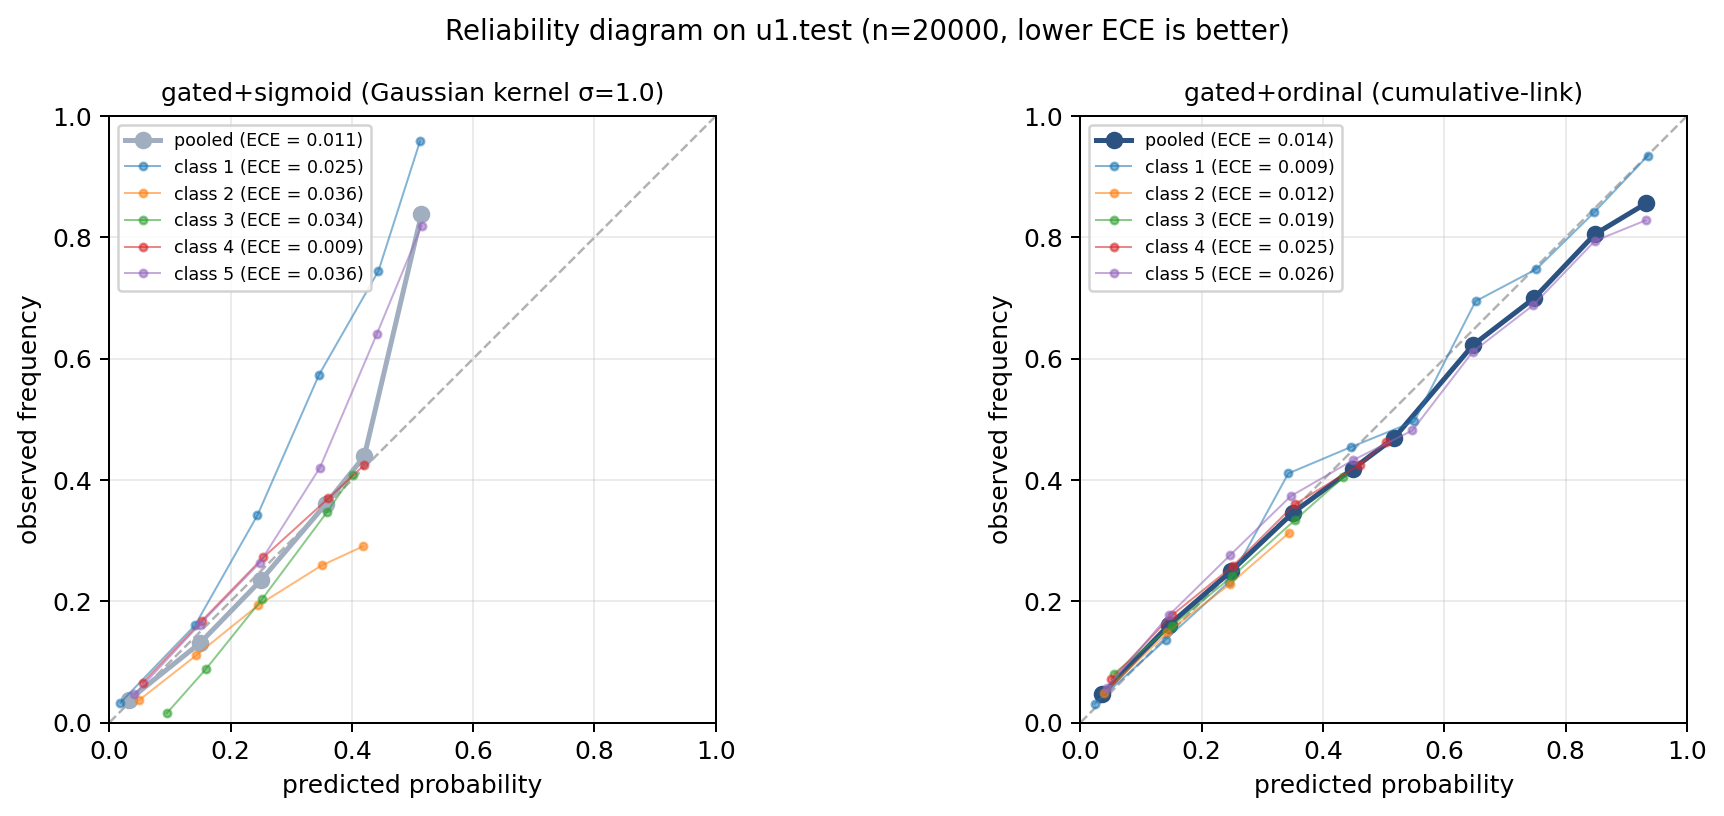
\includegraphics[width=\linewidth]{figures/reliability_curves_white.png}
\caption{Reliability diagrams on \texttt{u1.test}. Gated$+$ordinal is better
calibrated on classes 1, 2, 3, and 5; kernelised gated$+$sigmoid wins only on
the dominant class~4.}
\label{fig:reliability}
\end{figure}

\paragraph{Where the ordinal head wins: extreme classes.}
Figure~\ref{fig:per_class_f1} reports per-class F1 on \texttt{u1.test}. The
ordinal head wins on the boundary classes: $+0.098$ F1 on class~1 and
$+0.035$ F1 on class~5; classes 2--4 are within $\pm0.015$. Macro-F1 lifts
from $0.341$ to $0.369$, driven mainly by recall on classes 1 and 5. This is
the per-class footprint of the calibration claim.

\begin{figure}[ht]
\centering
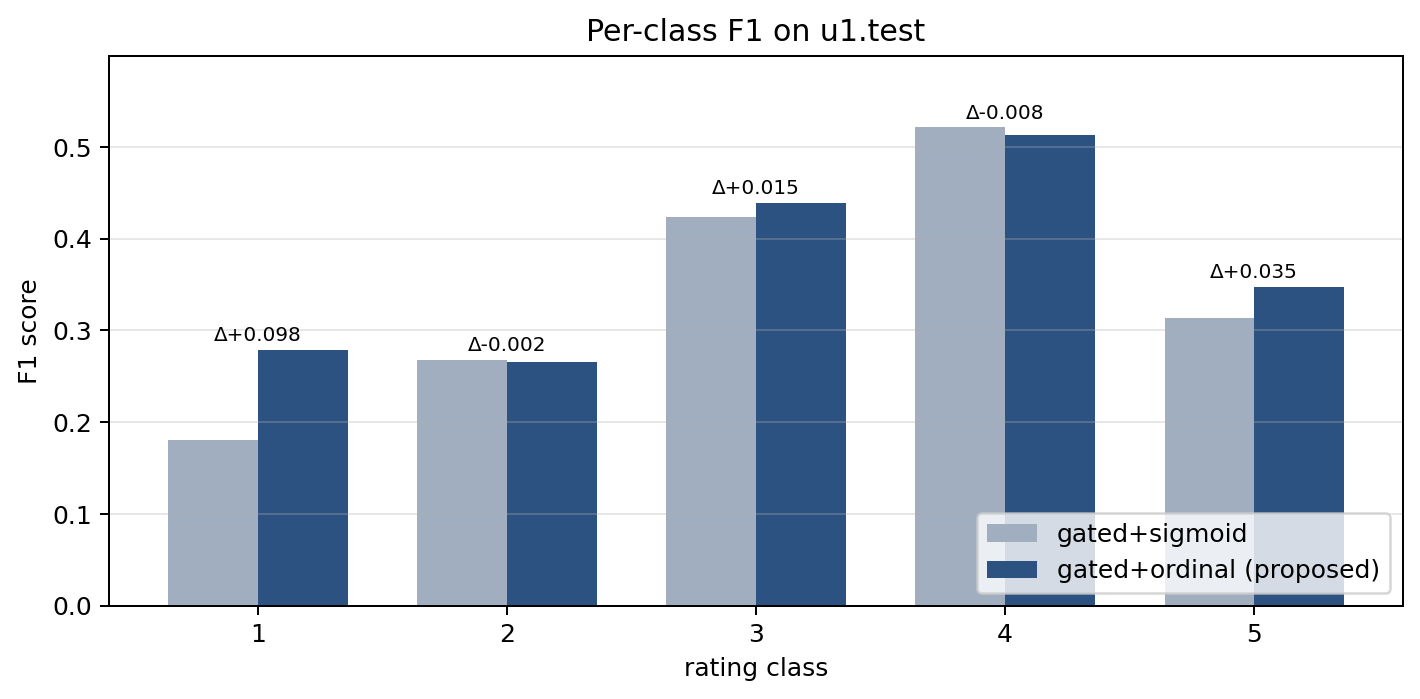
\includegraphics[width=0.66\linewidth]{figures/per_class_f1_white.png}
\caption{Per-class F1 on \texttt{u1.test} for the same gated backbone with
sigmoid vs.\ ordinal heads. The ordinal head wins on the extreme classes
(1 and 5) where the cumulative-link thresholds carry boundary information;
classes 2--4 are within seed-level noise.}
\label{fig:per_class_f1}
\end{figure}

Sensitivity checks supported $d=128$ and $\lambda=10^{-5}$: increasing to
$d=256$ improved RMSE by only $0.0024$ at $+34\%$ wall time, while
$\lambda=10^{-4}$ overregularised by $0.0080$ RMSE.

\subsection{Embedding visualisation}
\label{sec:viz}
We extract the post-fusion representations $p'_u$ and $q'_i$ from a single
gated$+$ordinal model trained on the \texttt{u1} split (seed $42$, test RMSE
$0.9165$), and project them to
$\mathbb{R}^2$ via three classical manifold methods: PCA~\cite{jolliffe2002pca}
(linear, variance
preserving), classical MDS (linear, distance preserving), and
IsoMap~\cite{tenenbaum2000isomap} (nonlinear, geodesic distance preserving,
$k=15$ neighbours). To keep figures legible, we sample $\approx\!200$ users
balanced across the six most common occupations ($+\!$ ``rest''), and
$\approx\!200$ items balanced across the six most common dominant genres
($+\!$ ``rest''). Cluster quality is measured by the silhouette score with
respect to the categorical labels.

\begin{figure}[ht]
\centering
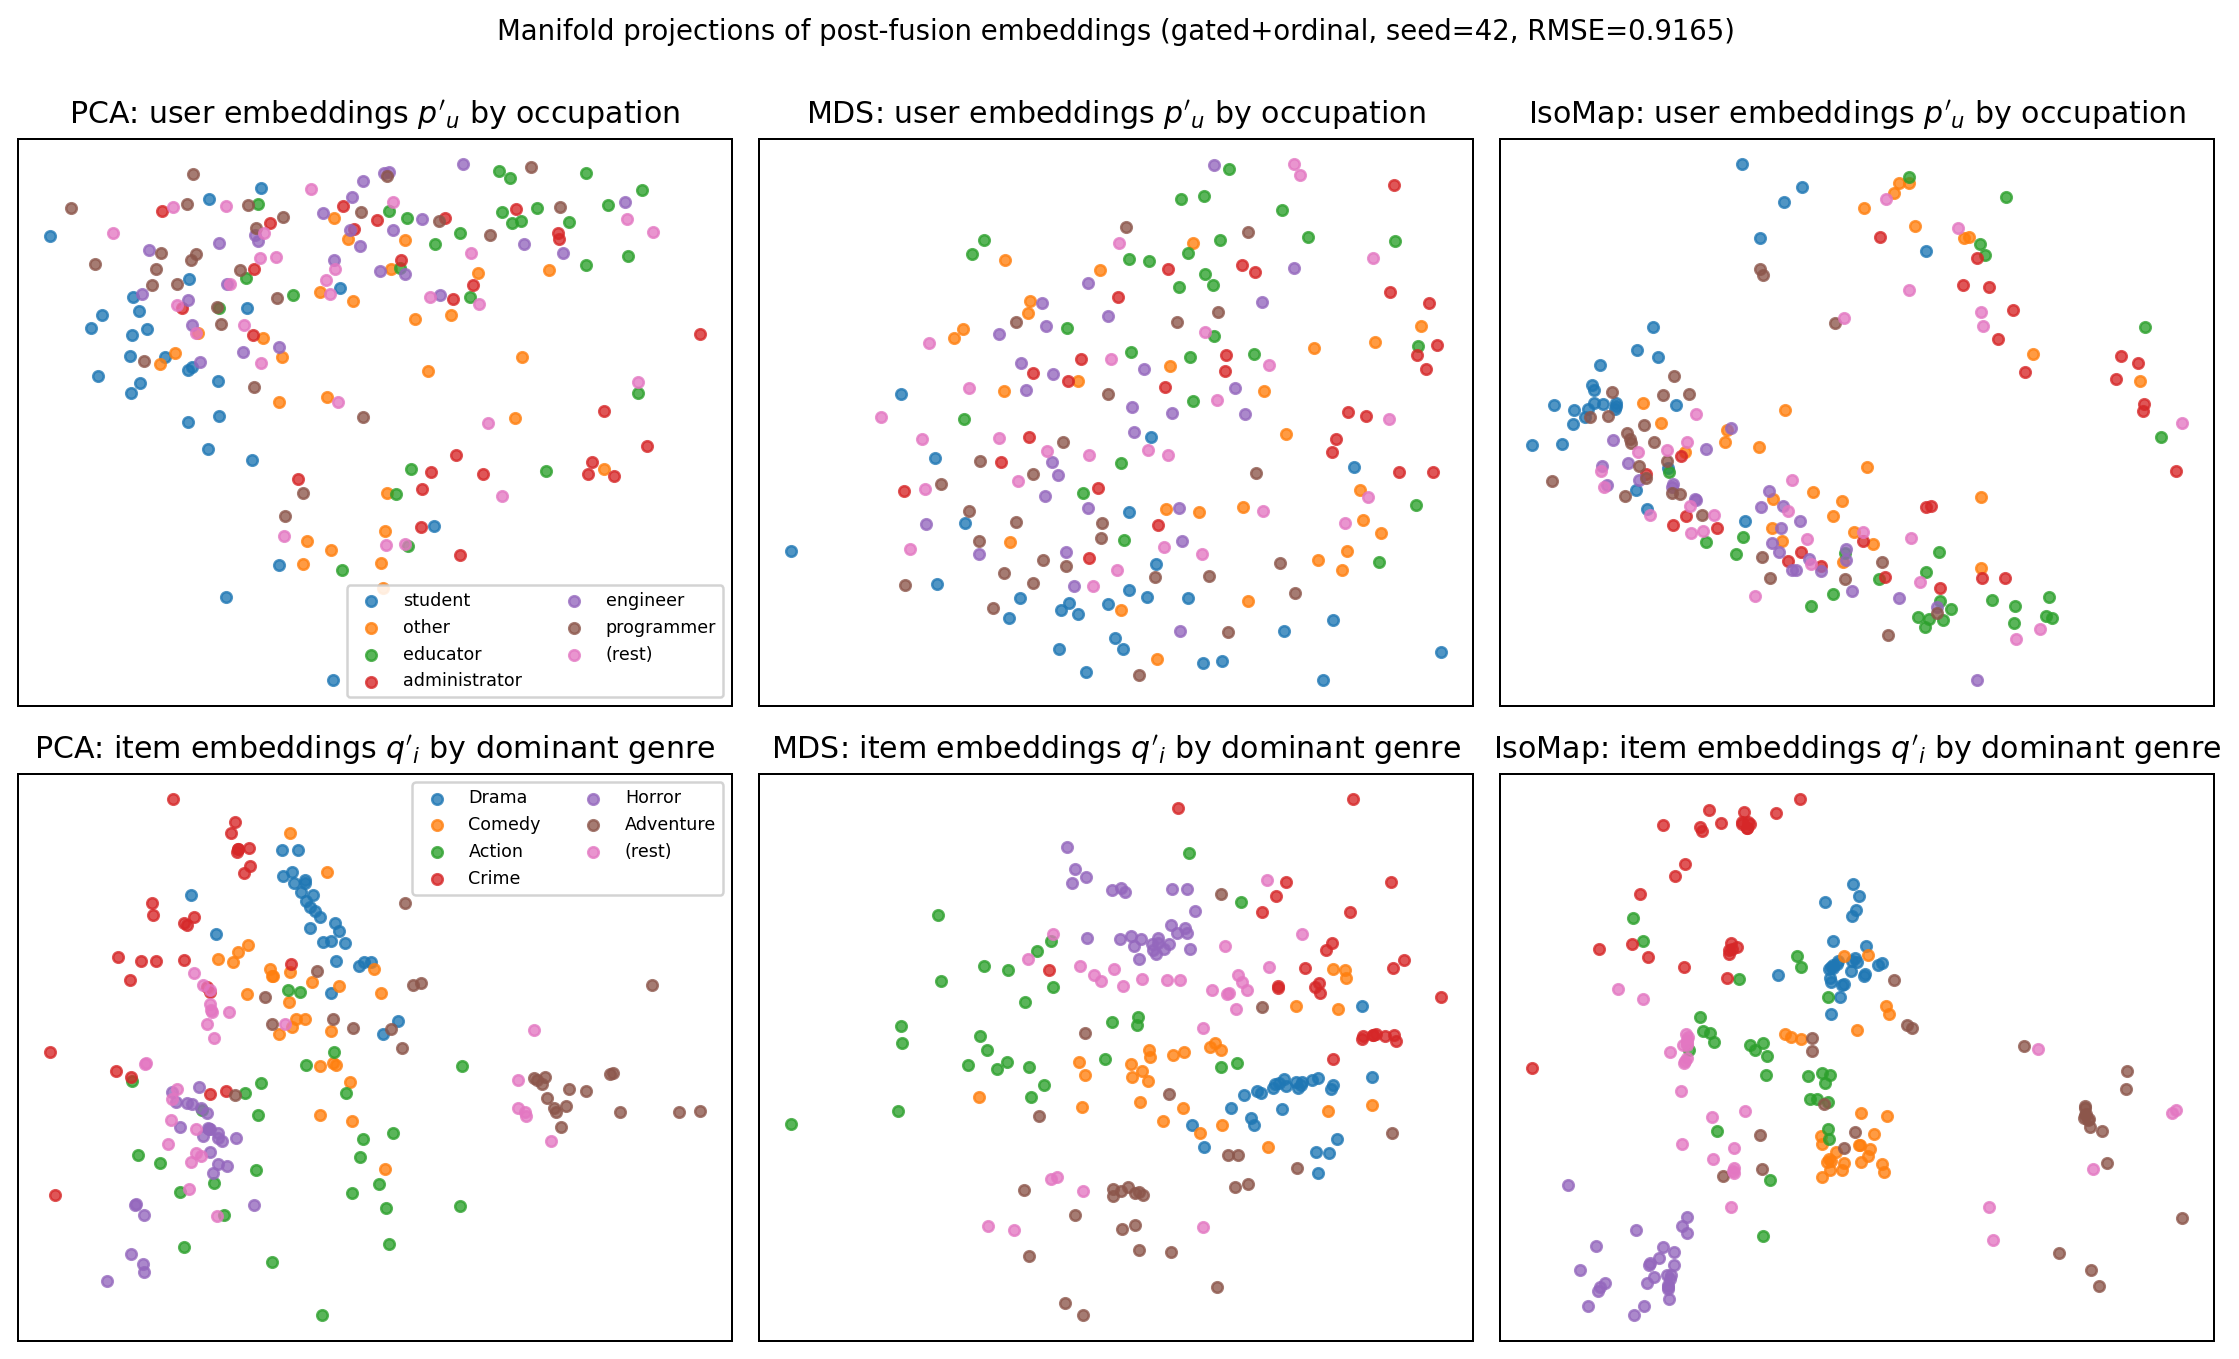
\includegraphics[width=0.86\linewidth]{figures/manifold_grid_white.png}
\caption{Two-dimensional projections of the post-fusion user
representations $p'_u$ (top, coloured by occupation) and item
representations $q'_i$ (bottom, coloured by dominant genre). Columns show
PCA, classical MDS, and IsoMap with $k=15$ neighbours. Item-side genre
structure is recovered most clearly by IsoMap; user-side occupation
structure is present in the high-dimensional space but does not survive
projection to two dimensions.}
\label{fig:manifold}
\end{figure}

\begin{table}[ht]
\centering
\caption{Silhouette scores in the full 128-dimensional space (HD) and after
projection to two dimensions, with respect to occupation labels (users) and
dominant genre labels (items).}
\label{tab:silhouette}
\begin{tabular}{lcccc}
\toprule
& HD ($d=128$) & 2D PCA & 2D MDS & 2D IsoMap \\
\midrule
$p'_u$ by occupation & $+0.0848$ & $-0.107$ & $-0.103$ & $-0.114$ \\
$q'_i$ by dominant genre & $+0.1930$ & $+0.048$ & $+0.137$ & $+0.232$ \\
\bottomrule
\end{tabular}
\end{table}

The model learns side-information structure without an auxiliary
classification loss. Item-side genre structure is clearer than user-side
occupation structure in 128-D ($+0.193$ vs $+0.085$), and it survives nonlinear
projection better than linear projection (IsoMap $+0.232$ vs PCA $+0.048$).
Occupation information is present in high dimension but does not compress
cleanly into two dimensions.

\subsection{Gate behaviour and cold-start regime}
\label{sec:coldstart}

\paragraph{Per-user trajectory.}
We stratify test predictions by the corresponding user's training activity
$|R_u|$ into five buckets and compare gated$+$ordinal against
additive$+$ordinal.

\begin{table}[ht]
\centering
\caption{Cold-start RMSE breakdown by user activity. Negative $\Delta$ means
additive fusion wins on that bucket.}
\label{tab:coldstart}
\begin{tabular}{lrrrrr}
\toprule
$|R_u|$ bucket & $<\!30$ & $30$--$59$ & $60$--$119$ & $120$--$239$ & $\ge\!240$ \\
\midrule
gated RMSE      & $0.9799$ & $0.9649$ & $0.8841$ & $0.8896$ & $0.9200$ \\
additive RMSE   & $0.9803$ & $0.9768$ & $0.8929$ & $0.8946$ & $0.9128$ \\
$\Delta$ (add. $-$ gated) & $+0.0004$ & $+0.0119$ & $+0.0088$ & $+0.0051$ & $-0.0071$ \\
mean $g_u$ & $0.246$ & $0.256$ & $0.263$ & $0.268$ & $0.291$ \\
mean $g_i$ & $0.316$ & $0.317$ & $0.316$ & $0.317$ & $0.316$ \\
\bottomrule
\end{tabular}
\end{table}

The cold-start table complicates the aggregate result. Gated fusion is strongest
for mid-activity users, ties on the coldest bucket, and reverses for the 14
most active users. Its gain is therefore not uniform across activity regimes,
even though it wins on the overall mean.

\subsection{Gate interpretability}
Aggregate gate values disguise a useful per-dimension pattern. For the trained
gated$+$ordinal model on \texttt{u1}, Figure~\ref{fig:gate_perdim} sorts each
dimension by its population-mean gate value. The user-side gate spans
$[0.002,0.984]$ with mean $0.263$; the item-side gate spans $[0.002,0.992]$
with mean $0.317$. Only about one fifth of dimensions sit above the zero-init
value of $0.5$, so the fusion mechanism is not simply averaging ID embeddings
and side features. Most dimensions specialise toward the ID pathway, while a
smaller subset opens strongly toward side information.

\begin{figure}[ht]
\centering
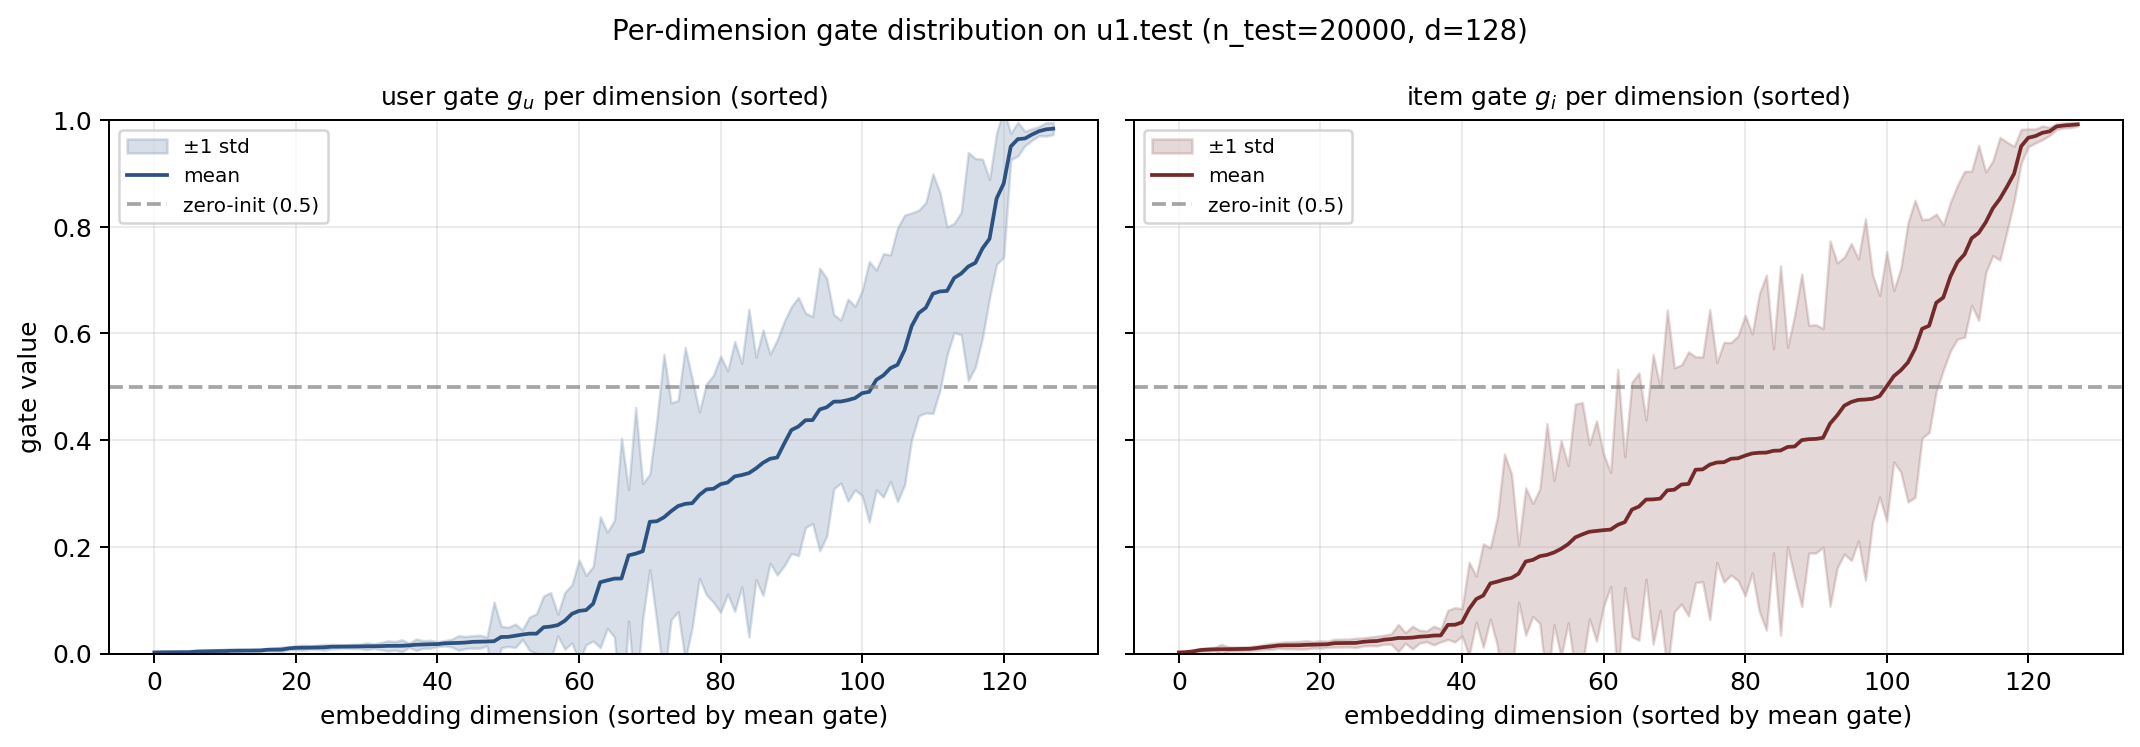
\includegraphics[width=0.86\linewidth]{figures/gate_distribution_white.png}
\caption{Per-dimension gate distribution on \texttt{u1.test}, sorted by mean.
The shaded band is $\pm 1$ std across the test population.}
\label{fig:gate_perdim}
\end{figure}

\subsection{Scale-up to MovieLens-1M}
\label{sec:ml1m}
To check scale, we run the three most informative cells on MovieLens-1M
($1{,}000{,}209$ ratings) under a deterministic random $80/10/10$ split. All
other settings match the MovieLens-100K experiments, and each cell averages the
same three training seeds.

\begin{table}[ht]
\centering
\caption{Scale-up to MovieLens-1M, random $80/10/10$ split, mean $\pm$ std over
three seeds.}
\label{tab:ml1m}
\resizebox{\linewidth}{!}{%
\begin{tabular}{llcccc}
\toprule
Fusion & Head & RMSE & MAE & Accuracy & NLL \\
\midrule
none      & sigmoid & $0.8567\pm0.0008$ & $0.6782\pm0.0007$ & $0.4480\pm0.0005$ & --- \\
gated     & sigmoid & $0.8502\pm0.0003$ & $0.6695\pm0.0001$ & $0.4579\pm0.0002$ & --- \\
\textbf{gated} & \textbf{ordinal} & $\mathbf{0.8481\pm0.0006}$ & $\mathbf{0.6630\pm0.0010}$ & $\mathbf{0.4654\pm0.0014}$ & $\mathbf{1.1842\pm0.0013}$ \\
\bottomrule
\end{tabular}%
}
\end{table}

The ordering matches MovieLens-100K: gated fusion improves RMSE over no fusion,
and adding the ordinal head improves it again. The larger data set also tightens
seed variance, consistent with more stable gate training.

\subsection{Reproducibility}
The code path is intentionally small enough to audit. All reported tables and
figures are regenerated from archived JSON/CSV outputs or from the scripts in
Table~\ref{tab:repro}. Each script records the model configuration, split,
seed, and metric outputs used in the paper. The reported ablation uses training
seeds $\{42,43,44\}$ on each canonical split and fixes the validation-split seed
so split variance is not mixed with model-initialisation variance.

\begin{table}[ht]
\centering
\caption{Core reproduction scripts. Wall times are approximate on M1 Pro CPU.}
\label{tab:repro}
\resizebox{\linewidth}{!}{%
\begin{tabular}{lll}
\toprule
Result & Script & Time \\
\midrule
Main ablation, 6 cells, 5 splits & \texttt{run\_multisplit.py} & $\sim$60 min \\
Baseline sanity check & \texttt{run\_baselines.py} & $\sim$5 min \\
Sensitivity curves & \texttt{run\_sensitivity.py} & $\sim$15 min \\
Class F1 and reliability & \texttt{run\_classmetrics.py}, \texttt{run\_reliability.py} & $\sim$4 min \\
Embedding and cold-start diagnostics & \texttt{run\_visualization.py}, \texttt{run\_coldstart.py} & $\sim$3 min \\
MovieLens-1M scale-up & \texttt{run\_ml1m.py} & $\sim$85 min \\
\bottomrule
\end{tabular}
}
\end{table}

\subsection{Discussion}
The ablation paints a sharper picture than the headline number alone. Gated
fusion accounts for most of the empirical RMSE change; the ordinal head provides
native probability estimates cheaply but does not help RMSE on its own. This
interaction suggests that ordinal heads are most useful here when paired with
side-information mechanisms, not as a stand-alone substitute for them.

\paragraph{Limitations.}
The benchmark is small ($100$K ratings); the side information is limited to
demographics and genres; and the ordinal head is calibrated to the
rating-class marginal but does not model per-user heteroscedasticity.

\section{Conclusion}
\label{sec:conclusion}
We presented a calibration recipe for cumulative-link collaborative filtering:
initialise the monotone thresholds from the training-set rating quantiles,
parameterise their spacing through a softplus-inverse, and exclude them from
$L_2$ regularisation. Paired with per-dimension gated side information, the
resulting model attains RMSE $0.9124\pm0.0036$ and NLL $1.2584$ across the five
MovieLens-100K splits, improving the across-split mean over both a no-fusion MF
analogue and additive fusion. The main lesson is that gating drives the RMSE
gain, while the ordinal head gives calibrated probabilities and better
boundary-class behaviour at negligible parameter cost. MovieLens-1M repeats the
same ordering at larger scale, and the cold-start breakdown shows that the
gated advantage is strongest in the mid-tail rather than uniform across users.

\bibliographystyle{plain}
\bibliography{refs}

\end{document}
